\documentclass[11pt,a4paper]{article}
\usepackage[utf8]{inputenc}
\usepackage[danish]{babel}
\usepackage{amsmath, amssymb, amsfonts}
\usepackage{graphicx}
\usepackage{tikz}
\usepackage{listings}
\usepackage{xcolor}

\usepackage{mathtools}



% Konfiguration af udseende for kode-blokken (uden at loade eksterne sprogfiler)
\lstdefinestyle{mystyle}{
    basicstyle=\small\ttfamily,
    breaklines=true,
    frame=single,
    backgroundcolor=\color{gray!5},
    keywordstyle=\color{blue},
    commentstyle=\color{green!50!black},
    columns=fullflexible
}

\begin{document}

% --- SIDE 1 ---
\section*{Eks. på beregn. af SVT ved qubitization}

$\tilde{P}(x) = x^2$ opfylder:
\begin{itemize}
    \item $P_{\mathbb{R}}$ har parity-($d \pmod 2$), and
    \item for all $x \in [-1, 1]: |P_{\mathbb{R}}(x)| \leq 1$.
\end{itemize}
\hfill $\left( \begin{smallmatrix} (i) & \deg(P) \leq k \text{ and } \deg(Q) \leq k-1 \\ (ii) & P \text{ has parity-}(k \pmod 2) \text{ and } Q \text{ has parity-}(k-1 \pmod 2) \end{smallmatrix} \right)$

Nu bruges lemma 6 på på $1 - \tilde{P}^2(x) = 1 - x^4$ som $(*)$ foreslår:
\[ 1 - x^4 = B^2(x) + (1 - x^2) C^2(x) \]
for at finde $P, Q \in \mathbb{C}[x]$ så
\[ (iv) \quad \forall x \in [-1, 1] : |P(x)|^2 + (1 - x^2)|Q(x)|^2 = 1 \]
er opfyldt.

Der gælder altså ifølge lemma 6 at
\begin{align*}
    &\text{grad } B \leq 2, \quad \text{grad } C \leq 1, \quad C \text{ ulige}, \quad B \text{ lige} \\
    &B = ax^2 + b, \quad C = \alpha x \quad \Rightarrow \\
    &a^2x^4 + b^2 + 2abx^2 + (1 - x^2) \alpha^2 x^2 \\
    &x^4(a^2 - \alpha^2) + x^2(2ab + \alpha^2) + b^2 = 1 - x^4 \Rightarrow \\
    &2ab + \alpha^2 = 0, \quad b^2 = 1, \quad a^2 - \alpha^2 = -1 \Rightarrow \alpha^2 = a^2 + 1 \\
    &2ab + 1 + a^2 = 0 \\
    &b = 1 \Rightarrow a^2 + 2a + 1 = 0 \Rightarrow d = 4 - 4 \cdot 1 \cdot 1 = 0 \Rightarrow a = \frac{-2}{2} = -1 \Rightarrow \alpha = \pm \sqrt{2} \\
    &b = -1 \Rightarrow a^2 - 2a + 1 = 0 \Rightarrow d = 4 - 4 \cdot 1 \cdot 1 = 0 \Rightarrow a = 1
\end{align*}

Dvs. man har:
\begin{gather*}
    B = \mp x^2 \pm 1, \quad C = \pm \sqrt{2}x \\
    P(x) = x^2 + i(\mp x^2 \pm 1), \quad Q(x) = \pm \sqrt{2}i x
\end{gather*}

Betingelsen (iv) tjekkes:
\begin{align*}
    x^4 + (1 - x^2)^2 + (1 - x^2)(\sqrt{2}x)^2 &= \\
    x^4 + (x^4 + 1 - 2x^2) + (1 - x^2)2x^2 &= \\
    2x^4 + 1 - 2x^2 + 2x^2 - 2x^4 &= 1
\end{align*}

\newpage

% --- SIDE 2 ---
Nu anvendes algoritmen i Thm. 3 på
\begin{align*}
    P(x) &= x^2 + i(x^2 - 1) = (1+i)x^2 - i \\
    Q(x) &= \sqrt{2}ix
\end{align*}
til at finde $\Phi$:

Ifølge bevist for thm. 3 skal $e^{2i\phi_k} = \frac{p_\ell}{q_{\ell-1}}$ for $k=2$ \\
(Bemærk at $|1+i| = \sqrt{2} = |\sqrt{2}i|$ så højsteggrads led er lige store)

\[ e^{2i\phi_2} = \frac{1+i}{\sqrt{2}i} = \frac{1-i}{\sqrt{2}} \]
dvs $e^{i\theta} = \frac{1}{\sqrt{2}} - i \frac{1}{\sqrt{2}}$

\begin{center}
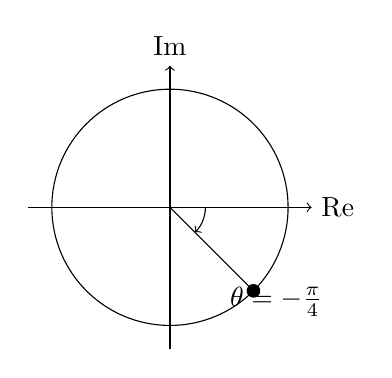
\begin{tikzpicture}[scale=1.5]
    \draw[->] (-1.2,0) -- (1.2,0) node[right] {Re};
    \draw[->] (0,-1.2) -- (0,1.2) node[above] {Im};
    \draw (0,0) circle (1);
    \filldraw (0.707,-0.707) circle (1.5pt);
    \draw (0,0) -- (0.707,-0.707);
    \node at (0.9,-0.8) {$\theta = -\frac{\pi}{4}$};
    \draw[->] (0.3,0) arc (0:-45:0.3);
\end{tikzpicture}
\end{center}

\[ \theta = -\frac{\pi}{4} \Rightarrow 2\phi_2 = -\frac{\pi}{4} \Rightarrow \phi_2 = -\frac{\pi}{8} \]

Nu defineres
\begin{align*}
    \tilde{P}(x) &= e^{-i\phi_k} x P(x) + e^{i\phi_k}(1-x^2)Q(x) = e^{-i\phi_k}\left( x P(x) + \frac{p_\ell}{q_{\ell-1}}(1-x^2)Q(x) \right) \\
    \tilde{Q}(x) &= e^{i\phi_k} x Q(x) - e^{-i\phi_k} P(x) = e^{-i\phi_k} \left( \frac{p_\ell}{q_{\ell-1}} x Q(x) - P(x) \right)
\end{align*}
$\tilde{P}$ og $\tilde{Q}$ skulle meget gerne have lavere grad end $P$ hhv. $Q$:

\begin{align*}
    \tilde{Q}(x) &= e^{i\pi/8} \left( \frac{1-i}{\sqrt{2}} x Q(x) - P(x) \right) \\
    &= e^{i\pi/8} \left( (1-i)i x^2 - (1+i)x^2 - i \right) = \\
    &= e^{i\pi/8} \left( (1+i)x^2 - (1+i)x^2 - i \right) = e^{i\pi/8} e^{-i\pi/2} \text{ (fejl i ms, rettet til: )} = e^{-i3\pi/8} \\
    \tilde{P}(x) &= e^{i\pi/8} \left( x((1+i)x^2 - i) + \frac{1-i}{\sqrt{2}}(1-x^2)i\sqrt{2}x \right) \\
    &= e^{i\pi/8} \left( (1+i)x^3 - ix + (1+i)x - (1+i)x^3 \right)
\end{align*}

\newpage

% --- SIDE 3 ---
\[ = e^{i\pi/8} (-ix + x + ix) = e^{i\pi/8}x \]

Algoritmen fortsættes med $P_1(x) = e^{i\pi/8}x$, $Q_0 = e^{i5\pi/8}$
\
\[ 2\phi_1 = -\pi/2 \Rightarrow \phi_1 = -\pi/4 \]

\begin{align*}
    \tilde{Q}(x) &= e^{i\pi/4} (e^{i\pi/2} x e^{i5\pi/8} - e^{i5\pi/8}x) = 0 \\
    \tilde{P}(x) &= e^{i\pi/4} (x^2 e^{i\pi/8} + e^{i\pi/2}(1-x^2)e^{i5\pi/8}) \\
    &= e^{i\pi/4}(e^{i\pi/8}) = e^{i3\pi/8} = e^{i\phi_0} \Rightarrow \phi_0 = 3\pi/8
\end{align*}

Altså har man:
\[ \Phi = (3\pi/8, -\pi/4, -\pi/8) \]

Det skal nu vises at:
\begin{gather*}
    W(x) = \begin{bmatrix} x & i\sqrt{1-x^2} \\ i\sqrt{1-x^2} & x \end{bmatrix} \\
    e^{i\phi_0 \sigma_z} \prod_{j=1}^k (W(x) e^{i\phi_j \sigma_z}) = \begin{bmatrix} P(x) & iQ(x)\sqrt{1-x^2} \\ iQ^*(x)\sqrt{1-x^2} & P^*(x) \end{bmatrix}
\end{gather*}

Jeg tjekker med Maple:
\begin{lstlisting}[style=mystyle]
restart:
with(LinearAlgebra):
with(Student[LinearAlgebra]):
interface(rtablesize=infinity):

W(x) := Matrix([[x, I*sqrt(1-x^2)], [I*sqrt(1-x^2), x]]):
Phi := [3*Pi/8, -Pi/4, -Pi/8]:
Z := Matrix([[1, 0], [0, -1]]):
R0 := MatrixExponential(I*Phi[1]*Z):
R1 := MatrixExponential(I*Phi[2]*Z):
R2 := MatrixExponential(I*Phi[3]*Z):

simplify(R0 . W(x) . R1 . W(x) . R2)
\end{lstlisting}

\begin{center}
\fbox{$\begin{bmatrix} (1+i)x^2-1 & -x\sqrt{2}\sqrt{-x^2+1} \\ x\sqrt{2}\sqrt{-x^2+1} & 1+(1-i)x^2 \end{bmatrix}$}
\end{center}
... hvor det ses at passe

\newpage

% --- SIDE 4 ---
Nu anvendes $\Phi$ på block encodingen
\[ U = \begin{bmatrix} X & 0 \\ 0 & I \end{bmatrix} \]

Alt. phase mod seq er
\

I dette tilfælde:
\

Først skal findes ny $\tilde{\Phi}$:
\begin{gather*}
    \phi_1 := \phi'_0 + \phi'_d + (d-1)\frac{\pi}{2} \text{ and for all } j \in \{2, 3, \dots, d\} \text{ setting } \phi_j := \phi'_{j-1} - \frac{\pi}{2} \\
    \tilde{\phi}_1 = \frac{3\pi}{8} + \left( -\frac{\pi}{8} \right) + (2-1)\pi/2 = \frac{3\pi}{8} - \frac{\pi}{8} + \frac{4\pi}{8} = \frac{6\pi}{8} = \frac{3\pi}{4} \\
    \tilde{\phi}_2 = -\frac{\pi}{4} - \frac{\pi}{2} = -\frac{3\pi}{4}
\end{gather*}




\section{Initialisering og Definitioner}
Definition af qubitization-operatoren $W(x)$ og de fundamentale Pauli-matricer:
\begin{equation}
W(x) \coloneqq \begin{bmatrix} x & i\sqrt{1-x^2} \\ i\sqrt{1-x^2} & x \end{bmatrix}
\end{equation}

\begin{equation}
Z = \begin{bmatrix} 1 & 0 \\ 0 & -1 \end{bmatrix}, \quad 
Y = \begin{bmatrix} 0 & -i \\ i & 0 \end{bmatrix}, \quad 
X = \begin{bmatrix} 0 & 1 \\ 1 & 0 \end{bmatrix}
\end{equation}

\section{Polynomiel Transformation (QSP)}
Med faserne $\varphi = \langle \frac{3\pi}{8}, -\frac{\pi}{4}, -\frac{\pi}{8} \rangle$ beregnes produktet $R_0 \cdot W(x) \cdot R_1 \cdot W(x) \cdot R_2$:
\begin{equation}
\begin{bmatrix}
(1+i)x^2 - i & -x\sqrt{2}\sqrt{-x^2+1} \\
x\sqrt{2}\sqrt{-x^2+1} & i + (1-i)x^2
\end{bmatrix}
\end{equation}

Ved brug af alternativ operator $R(x) = \begin{bmatrix} x & \sqrt{1-x^2} \\ \sqrt{1-x^2} & -x \end{bmatrix}$ og faserne $\varphi_1 = \frac{3\pi}{4}$, $\varphi_2 = -\frac{3\pi}{4}$ fås:
\begin{equation}
\begin{bmatrix}
(1+i)x^2 - i & (1+i)x\sqrt{-x^2+1} \\
(-1+i)x\sqrt{-x^2+1} & i + (1-i)x^2
\end{bmatrix}
\end{equation}

\section{SVT af diagonalmatrix}
For $A = \text{diag}(0.6, 0.3)$ konstrueres blok-kodningen $U_A$:
\begin{equation}
U_A = \begin{bmatrix} 
 0.6 & 0 &  0.8 &  0 \\ 
 0 &  0.3 &  0 &  0.9539 \\ 
 0.8 &  0 & -0.6 & 0 \\ 
 0 &  0.9539 & 0 & -0.3 
\end{bmatrix}
\end{equation}

Beregning af transformeret unitær $U_{\text{transf}} = U_1 \cdot U_A^\dagger \cdot U_2 \cdot U_A$:
De singulære værdier for $\Pi \cdot U_{\text{transf}} \cdot \Pi$ er:
\begin{equation}
\sigma(U_{\text{transf}}) \approx \{0.9145, 0.7343\}
\end{equation}

\section{SVT af ikke-diagonalmatrix}
En basis-transformation $Q = \exp(i \frac{\pi}{7} X)$ anvendes på $A$, hvilket giver $B = Q^{-1} A Q$:
\begin{equation}
B = \begin{bmatrix} 0.5435 & 0.1173i \\ -0.1173i & 0.3565 \end{bmatrix}, \quad \sigma(B) = \{0.6, 0.3\}
\end{equation}
Blok-kodningen $U_B$ og transformationen $U_{B,\text{transf}}$ giver samme singulære værdier som i det diagonale tilfælde.

\section{SVT med REELT polynomium}
For at opnå et reelt polynomium defineres de konjugerede transformationer:
\begin{align}
U_{1m} &= \exp(i \cdot (-\varphi_1) \cdot (2\Pi - E)) \\
U_{2m} &= \exp(i \cdot (-\varphi_2) \cdot (2\Pi - E))
\end{align}

Den kombinerede transformation beregnes som gennemsnittet:
\begin{equation}
\text{SVT}_{\text{reel}} = \Pi \cdot \left( \frac{U_{B,\text{transf}} + U_{B,\text{transf,conj}}}{2} \right) \cdot \Pi
\end{equation}

Resultatet giver de kvadrerede singulære værdier:
\begin{equation}
\text{SingularValues} \approx \begin{bmatrix} 0.3600 \\ 0.0900 \\ 0 \\ 0 \end{bmatrix}
\end{equation}
Hvilket svarer præcis til $0.6^2$ og $0.3^2$. Dette bekræfter, at realdelen af transformationen svarer til anvendelsen af det reelle polynomium $x^2$ på matrix-niveu.



\section*{Qubitization Worksheet}

$restart :$ \\
$with(LinearAlgebra) :$ \\
$with(Student[LinearAlgebra]) :$ \\
$interface(rtablesize = infinity) :$

\begin{equation}
W(x) \coloneqq \begin{bmatrix} x & I \cdot \sqrt{1-x^2} \\ I \cdot \sqrt{1-x^2} & x \end{bmatrix}
\end{equation}

$\phi \coloneqq \left\langle \frac{3 \cdot \pi}{8}, -\frac{\pi}{4}, -\frac{\pi}{8} \right\rangle :$

\begin{equation}
Z \coloneqq \begin{bmatrix} 1 & 0 \\ 0 & -1 \end{bmatrix}; \quad 
Y \coloneqq \begin{bmatrix} 0 & -I \\ I & 0 \end{bmatrix}; \quad 
X \coloneqq \begin{bmatrix} 0 & 1 \\ 1 & 0 \end{bmatrix};
\end{equation}

$R0 \coloneqq MatrixExponential(I \cdot \phi[1] \cdot Z) :$ \\
$R1 \coloneqq MatrixExponential(I \cdot \phi[2] \cdot Z) :$ \\
$R2 \coloneqq MatrixExponential(I \cdot \phi[3] \cdot Z) :$

\begin{equation}
simplify(R0 \cdot W(x) \cdot R1 \cdot W(x) \cdot R2) = 
\begin{bmatrix} 
(1+I)x^2 - I & -x\sqrt{2}\sqrt{-x^2+1} \\ 
x\sqrt{2}\sqrt{-x^2+1} & I + (1-I)x^2 
\end{bmatrix}
\end{equation}

$R(x) \coloneqq \begin{bmatrix} x & \sqrt{1-x^2} \\ \sqrt{1-x^2} & -x \end{bmatrix} :$

$\varphi1 \coloneqq \frac{3\pi}{8} - \frac{\pi}{8} + \frac{\pi}{2} = \frac{3\pi}{4}$ \\
$\varphi2 \coloneqq -\frac{\pi}{4} - \frac{\pi}{2} = -\frac{3\pi}{4}$

\begin{equation}
simplify(Rr1 \cdot R(x) \cdot Rr2 \cdot R(x)) = 
\begin{bmatrix} 
(1+I)x^2 - I & (1+I)x\sqrt{-x^2+1} \\ 
(-1+I)x\sqrt{-x^2+1} & I + (1-I)x^2 
\end{bmatrix}
\end{equation}

\subsection*{SVT af diagonalmatrix}

$A \coloneqq \begin{bmatrix} 0.6 & 0 \\ 0 & 0.3 \end{bmatrix}$

$A2 \coloneqq MatrixPower(E2 - A \cdot HermitianTranspose(A), 1/2) :$

\begin{equation}
UA \coloneqq \begin{bmatrix} 
0.6 & 0 & 0.8 & 0 \\ 
0 & 0.3 & 0 & 0.9539392014 \\ 
0.8 & 0 & -0.6 & 0 \\ 
0 & 0.9539392014 & 0 & -0.3 
\end{bmatrix}
\end{equation}

$\Pi \coloneqq \begin{bmatrix} 1 & 0 & 0 & 0 \\ 0 & 1 & 0 & 0 \\ 0 & 0 & 0 & 0 \\ 0 & 0 & 0 & 0 \end{bmatrix}; \quad 
E \coloneqq \begin{bmatrix} 1 & 0 & 0 & 0 \\ 0 & 1 & 0 & 0 \\ 0 & 0 & 1 & 0 \\ 0 & 0 & 0 & 1 \end{bmatrix}$

$U1 \coloneqq MatrixExponential(I \cdot \varphi1 \cdot (2\cdot\Pi - E)) :$ \\
$U2 \coloneqq MatrixExponential(I \cdot \varphi2 \cdot (2\cdot\Pi - E)) :$ \\
$Utransf \coloneqq simplify(U1 \cdot HermitianTranspose(U) \cdot U2 \cdot U)$

\begin{equation}
SingularValues(\Pi \cdot Utransf \cdot \Pi) = \begin{bmatrix} 0.9145551563 \\ 0.7343023898 \\ 0 \\ 0 \end{bmatrix}
\end{equation}

$(1+I)\cdot(0.6)^2 - I = 0.36 - 0.64I$ \\
$(1+I)\cdot(0.3)^2 - I = 0.09 - 0.91I$

\textit{Så ved at tage realdelen ser man at vi har kvadreret de singulære værdier ... men det dur vist kun for reelle værdier ....}

\subsection*{SVT af ikke-diagonalmatrix}

$Q \coloneqq MatrixExponential(I \cdot \frac{\pi}{7} \cdot X) :$ \\
$B \coloneqq simplify(MatrixInverse(Q) \cdot A \cdot Q)$

\begin{equation}
B = \begin{bmatrix} 0.5435234702 & 0.1172747224I \\ -0.1172747224I & 0.3564765298 \end{bmatrix}
\end{equation}

$SingularValues(B) = \begin{bmatrix} 0.6000000004 \\ 0.3000000000 \end{bmatrix}$

$UBTransf \coloneqq simplify(U1 \cdot HermitianTranspose(UB) \cdot U2 \cdot UB)$

\begin{equation}
SingularValues(\Pi \cdot UBTransf \cdot \Pi) = \begin{bmatrix} 0.9144397191 \\ 0.7343023900 \\ 0 \\ 0 \end{bmatrix}
\end{equation}

\textit{jeg forstår faktisk ikke hvad det er for en funkion af de sing værdier vi får frem ... TÆNK OVER DETTE!}

\subsection*{SVT med REELT polynomium}

$U1m \coloneqq MatrixExponential(I \cdot (-\varphi1) \cdot (2\cdot\Pi - E)) :$ \\
$U2m \coloneqq MatrixExponential(I \cdot (-\varphi2) \cdot (2\cdot\Pi - E)) :$ \\
$UBTransfConj \coloneqq simplify(U1m \cdot HermitianTranspose(UB) \cdot U2m \cdot UB)$

\begin{equation}
SingularValues\left( \Pi \cdot \left( \frac{UBTransfConj + UBTransf}{2} \right) \cdot \Pi \right) = \begin{bmatrix} 0.3600000001 \\ 0.09000000006 \\ 0 \\ 0 \end{bmatrix}
\end{equation}

\textit{He he .. her var de. Nu er deer totalt (næsten) styr på det.}





\end{document}


